% !TEX root = ../../main_netxpto.tex
\clearpage

\section{PSD Estimator}

\begin{refsection}

\begin{tcolorbox}	
	\begin{tabular}{p{2.75cm} p{0.2cm} p{10.5cm}} 	
		\textbf{Header File}   &:& psd\_estimator\_*.h \\
		\textbf{Source File}   &:& psd\_estimator\_*.cpp \\
		\textbf{Version}	   &:& 20180704 (Andoni Santos)
	\end{tabular}
\end{tcolorbox}

\subsection*{Input Parameters}

\begin{table}[H]
	\centering
	\begin{tabular}{|l|l|l|}
		\hline
		\textbf{Name}  		 & \textbf{Type}  & \textbf{Default Value}    	\\\hline
%		Confidence     		 & double         & 0.95              	\\\hline
		method				& enum				& WelchPgram			\\\hline
		ignoreInitialSamples & int				& 513					\\\hline
		windowType			 & WindowType     & Hanning			  	\\\hline
		measuredIntervalSize & int 			  & 2048				\\\hline
		segmentSize			 & int			  & 512					\\\hline
		overlapPercent 		 & int			  & 0.5					\\\hline
		filename			& string			& signals/PSD.txt	\\\hline
%		LowestMinorant & double         & $1\times10^{-10}$ \\ \hline
	\end{tabular}
\end{table}


\subsection*{Methods}

\subsection*{Input Signals}

\textbf{Number}: 1 or 2\\
\textbf{Type}: OpticalSignal or TimeContinuousAmplitudeContinuousReal

\subsection*{Output Signals}

\textbf{Number}: 1 or 2\\
\textbf{Type}: OpticalSignal or TimeContinuousAmplitudeContinuousReal

\subsection*{Functional Description}
This block accepts one OpticalSignal or TimeContinuousAmplitudeContinousReal signal
(or two real signals, an In-phase signal and a quadrature signal) and outputs
an exact copy of the input signals to the output. As it receives the input
signals, it saves until it has enough to perform a power spectral density
estimation, in W/Hz. The number of samples required to perform this estimation is defined
by the parameter \texttt{measuredIntervalSize}. After it has enough samples, it
proceeds to estimating the power spectral density of the signal through the
procedure chosen through the \texttt{method} parameter. Currently only one
method is available, the Welch periodogram (\texttt{WelchPgram}).

The result is then saved to the target file, specified by the \texttt{filename}
parameter. This file is updated each time that the number of samples is reached.
As the simulation continues to run, more samples are acquired and as the estimation is improved.

The file contains data divided in different lines, separated by "\textbackslash n", to simplify reading it with
external programs. The first line identifies the file as a PSD estimate.
The second line lists the number of segments averaged to obtain the estimated.
The third line identifies the chosen confidence interval.
The remaining lines are grouped in pairs, with the first line describing the
contents of the next one. These pairs contain, in order, the center of the
frequency bins, the PSD estimate, and the corresponding upper and lower
confidence bounds.
%The confidence intervals are calculated for the estimated PSD, taking into
%account that the PSD follows the Chi-Squared distribution with 2N degrees of
%freedom~\cite{jeruchim06}, with N being the number of segments used to estimate
%the PSD.

\begin{figure}[]
	\centering
	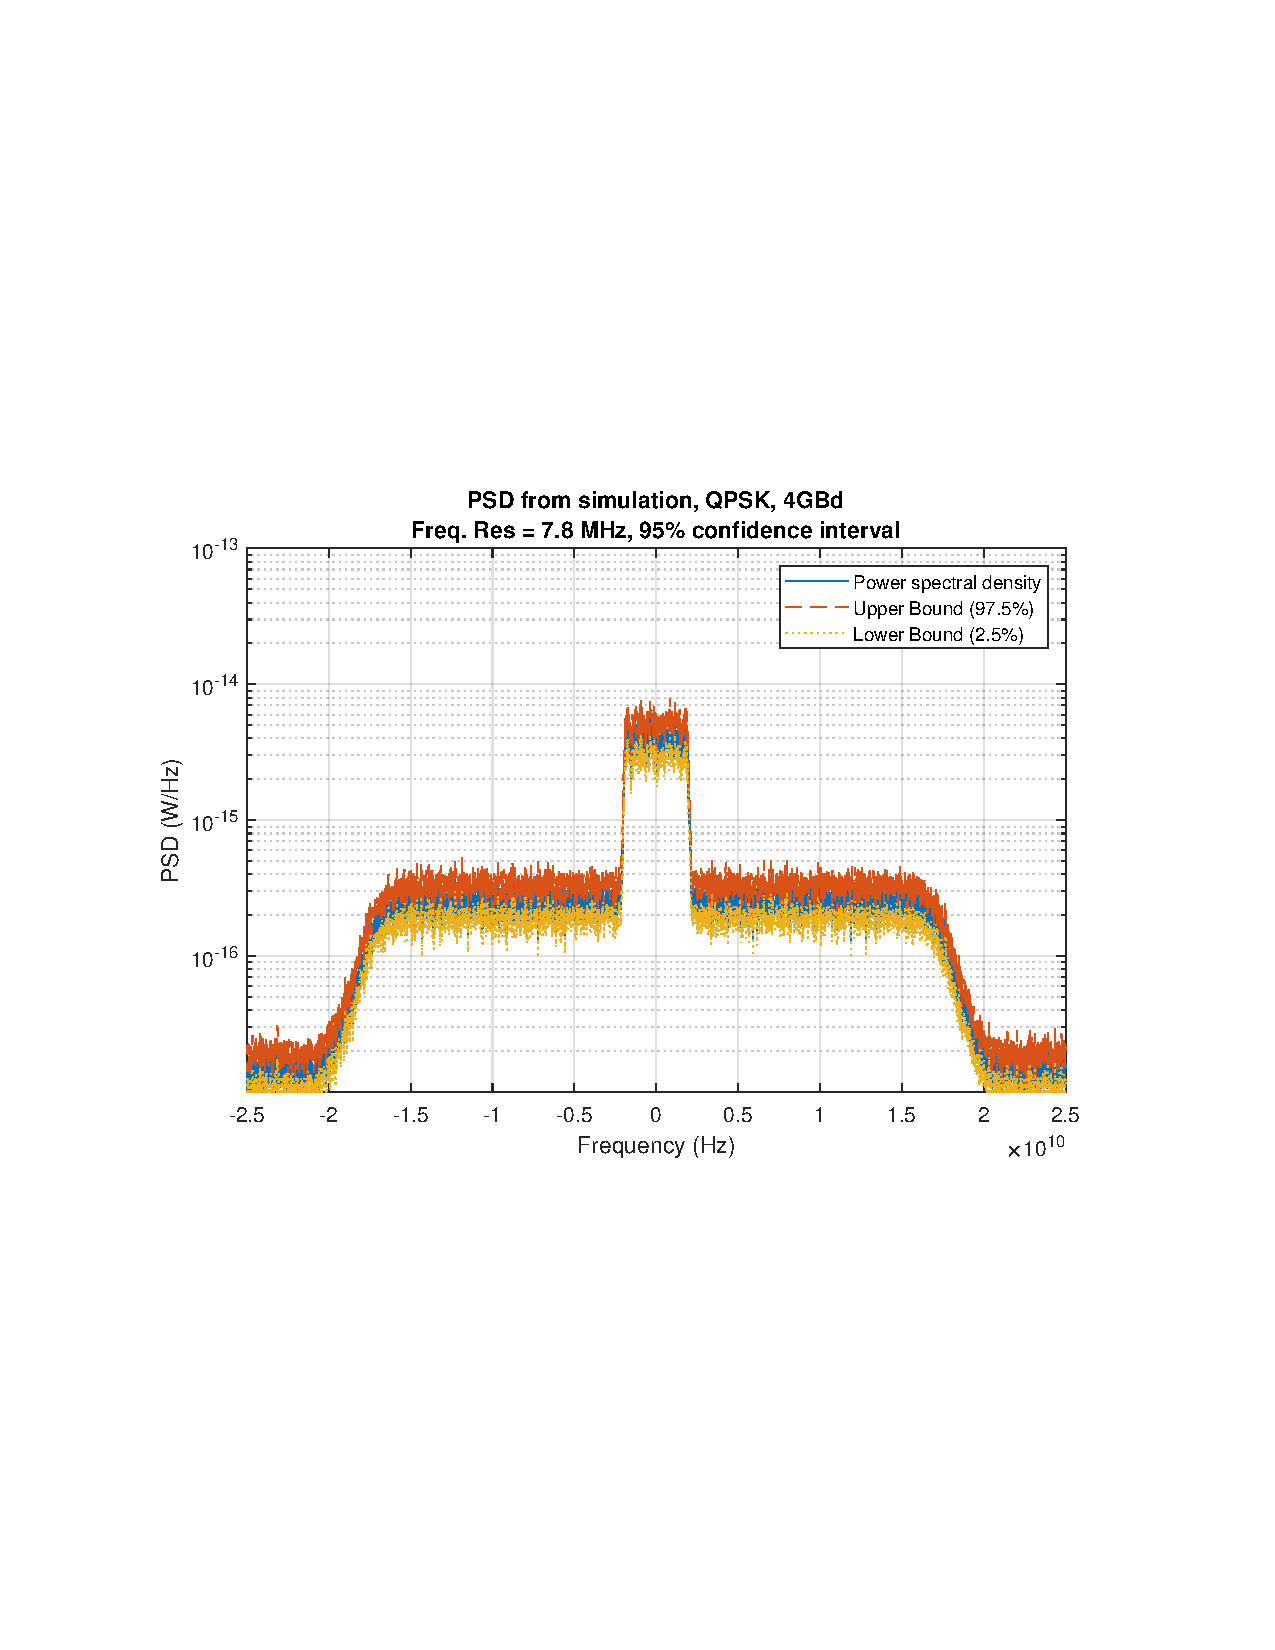
\includegraphics[clip, trim=2cm 8cm 2cm 8cm,width=0.7\textwidth]{./lib/psd_estimator/figures/qpskExample.pdf}
	\caption{Estimated power spectral density for a QPSK
	signal.\label{fig:psdExample}}
	
\end{figure}

\subsection*{Theoretical Description}\label{sec:psdEstTeor}
The techniques used for estimating the PSD are typically two, based on different
definitions of power spectral density. These are the periodogram (direct method) and the
correlogram (indirect method).

\subsubsection*{Periodogram}

It is also possible to define the PSD as follows~\cite{jeruchim06}:

\begin{equation}
	S_{XX}(f) = \lim_{T\to\infty} E \left[\hat{S}_{XX}\left(f, T\right)\right]
\end{equation}

\noindent with

\begin{equation}
	\hat{S}_{XX}(f,T) = \frac{{| X_T(f)|}^2}{T}
\end{equation}

\noindent and 

\begin{equation}
	X_T(f) = \int_0^T x(t) \exp(-j 2 \pi f t) dt
\end{equation}

$t{S}_{XX}(f,T)$ presents a natural estimation for the PSD, if the limiting and
expectation operations are omitted. This is called a periodogram. Its discrete
version is given by:

\begin{equation}
	\tilde{P}\left(f\right)  = \frac{1}{NT_s}{|X_N{\left(f\right)}|}^2
\end{equation}

\noindent with

\begin{equation}
	X_N\left(f\right) = T_s \sum_{n=0}^{N-1} X(n)
	\exp\left(-j2\pi f n T_s \right)
\end{equation}

$X_N(f)$ is the DFT of the observed data sequence, which can easily be
determined through FFt calculation.

To obtain the periodogram, the data needs to windowed. Windowing implies a
function that selects a certain portions of another function, either as is or
transforming it in a certain way.
Any finite observation is at least implicitly windowed with a
rectangular window, as it is a smaller set of the original function. Windows can
also modify the data in a given desired way. Any window necessarily alters the
true spectrum. The expected value of the periodograms is therefore different from the
true spectrum, instead providing a biased estimate. However, the periodogram is
asymptotically unbiased. This is because the effects of windowing, which are the
origin of the bias, disappear as the number of samples increases. For any window
$W(f)$, including the rectangular window, $|W(f)^2| \to
\delta(f)$ as the number of observations tends to infinity.

Also, for any periodogram, the standard deviation is at least as large as the
expected value of the spectrum, independently of the size of the observation.

Most common methods for obtaining periodograms try to avoid this issue.
One operation they resort to is the averaging of periodograms. This simply means
to obtain the average periodogram from a given set of periodograms obtained from
different signal sequences. The averaging of periodograms turn them into a
consistent estimator. In order to average the periodograms, the signal is
divided into smaller segments through windowing and periodograms are obtained
from different segments, in order to be averaged.

The two most common methods are the Bartlett periodogram and the Welch
periodogram. The Bartlett periodogram finds the average of nonoverlapping
signal segments obtained with a rectangular window. The Welch periodogram is
calculated by using segments with a certain amount of overlap, which are
obtained with other windows, typically Hann or Hamming.

\subsubsection*{Confidence intervals}
The periodogram is Chi-Square distributed~\cite{jeruchim06}. Therefore, the confidence interval
must be calculated accordingly. The confidence interval for a an estimated PSD
value $\hat{S}(f)$ is defined by~\cite{nsapplication255}

\begin{equation*}
	P\left( A < S(f) < B \right) = 1 - \alpha
\end{equation*}

\noindent where A and B are the bounds of the confidence interval, and $\alpha$ is the
probability of the true PSD value being outside the confidence interval. For a
given number of degrees of freedom, the interval's bounds are given by 

\begin{equation*}\label{eq:chsqBoundA}
	A = \frac{\nu \hat{S}(f)}{\chi^2_{1-\alpha/2}}
\end{equation*}
\begin{equation*}\label{eq:chsqBoundB}
	B = \frac{\nu \hat{S}(f)}{\chi^2_{\alpha/2}}
\end{equation*}

$\chi^2_{\alpha/2}$ can be obtained by finding the values at which the
chi-squared cumulative distribution function, for $\nu$ degrees of freedom, equals the desired 
probabilities. This function is calculated as~\cite{weisstein18csd}

\begin{equation}\label{eq:csqcdf}
	\text{CDF}(\chi^2) = \frac{\gamma \left(\nu/2, \chi^2/2\right)}
	{\Gamma\left(\nu/2\right)}
\end{equation}

\noindent where $\gamma\left(\nu/2,\chi^2i/2\right)$ is an incomplete gamma function and
	$\Gamma(\nu/2)$ is the gamma function. The values of $\chi^2$ needed for
	calculating A and B can be found by numerically evaluating~\ref{eq:csqcdf}
	to find the values which fit the desired probabilities. This is currently
	done using the bissection method, which provides an approximation better
	than most available tables 
	($\frac{|\alpha_{\text{calc}}-\alpha_{\text{desired}}|}{\alpha_{\text{desired}}}
	\le 10^{-6}$) in approximately 20 iterations.

	The confidence bounds are then calculated using
	equations~\ref{eq:chsqBoundA} and~\ref{eq:chsqBoundB}.



%\subsubsection{Correlogram}

%The PSD can be defined of a process can be defined as the Fourier transform of
%its autocorrelation function.



\subsection*{Known Issues}\label{psdestissues}
The current implementation for obtaining confidence intervals is susceptible to
underflow/overflow errors if the degrees of freedom grow too much, due to the calculation of the
incomplete gamma functions. This can mostly be avoided by making sure that
the segment size for calculating the periodogram is, at least, approximately
1/1000th of the total number of samples. 

\begin{equation*}
	\text{Segment\_size} \ge \frac{\text{NumberOfBits} \times
	\text{SamplesPerSymbol}}{1000 \times \text{BitsPerSymbol}}
\end{equation*}

In order to completely correct this
issue, two possibilities exist:
\begin{enumerate}
	\item Improve the algorithm in order to overcome
the overflow limitations, by using increased precision numeric types or some
other method;
\item By using a gaussian approximation for the distribution of the
periodogram, which is valid for larger degrees of freedom~\cite{jeruchim06}.
\end{enumerate}

%%%%%%%%%%%%%%%%%%%%%%%%%%%%%%%%%%%%%%%%%%%%%%%%%%%%%%%%%%%%%%%%%%%%%%%%%%%%%%%%%%%%%%%%%%%%%%%%%%%%%%%%%%%%
% References
%%%%%%%%%%%%%%%%%%%%%%%%%%%%%%%%%%%%%%%%%%%%%%%%%%%%%%%%%%%%%%%%%%%%%%%%%%%%%%%%%%%%%%%%%%%%%%%%%%%%%%%%%%%%


% bibliographic references for the section ----------------------------
\clearpage
\printbibliography[heading=subbibliography]
\end{refsection}
\addcontentsline{toc}{subsection}{Bibliography}
\cleardoublepage
% ---------------------------------------------------------------------
